%# -*- coding: utf-8-unix -*-
%%==================================================
%% chapter01.tex for SJTU Master Thesis
%%==================================================

%\bibliographystyle{sjtu2}%[此处用于每章都生产参考文献]
\chapter{绪论}
\label{chap:Pre}
\section{分组密码的概述}
分组密码是对称密码学的一个重要分之,是信息安全领域中极其重要的一部分,其研究内容主要包括分组密码的设计和分析这两个对立统一的方面。
一方面,密码设计者希望能够设计出抵抗所有已知密码攻击的密码算法;另一方面,密码分析者希望找到现有密码的某些安全缺陷。
这两方面的研究共同推动了分组密码理论的发展。

分组密码的设计理念源于Shannon于1949年发表的论文\emph{Communication Theory of Secrecy Systems}\cite{shannon1949communication},其公开研究开始于20世纪70年代提出的DES算法\citen{standard1977federal}。
分组密码理论和应用的飞速发展得益于上世纪末的美国AES计划本世纪初的NESSIE计划。

\section{分组密码的设计原理}
分组密码可以被认为是一个带密钥的置换,而每个密钥相当于从一类置换中选取一个置换。
分组密码的数学模型如下:
\begin{defn}[分组密码]
    记$\mathbb{F}_2$二元域,$\mathbb{F}_2^n$和$\mathbb{F}_2^m$分别为$\mathbb{F}_2^n$上的$n$和$m$维向量空间,$S_K\subseteq\mathbb{F}_2^m$,那么一个以$\mathbb{F}_2^n$为明文和密文空间、$S_K$为密钥空间的分组密码就可以表示为如下两个映射:
    $$E:\mathbb{F}_2^n\times S_K\rightarrow\mathbb{F}_2^n,\quad D:\mathbb{F}_2^n\times S_K\rightarrow\mathbb{F}_2^n$$
    上述两个映射满足对任意$k\in S_K$,$E(\cdot,k)$和$D(\cdot,k)$都是$\mathbb{F}_2^n$上的置换,并且互为逆置换。通常称$E(\cdot,k)$为固定密钥$k$时的加密函数,$D(\cdot,k)$为固定密钥$k$时的解密函数。
    上述模型中明文和密文的长度均为$n$,而密钥的长度为$l=log_2|S_K|$。
\end{defn}
而分组密码的设计就是找到一种算法,能使加密函数$E(\cdot,k)$和解密函数$D(\cdot,k)$十分容易计算,但从方程$y=E(x,k)$或$x=D(y,k)$中解出$k$十分困难。

分组密码的设计通常遵循如下两个原则:安全性原则和实现原则。安全性原则包含混淆原则、扩散原则和抗现有攻击原则;实现原则中包含了软件实现原则和硬件实现原则。本文中的研究将围绕分组密码的扩散原则进行讨论。

目前通用的分组密码算法都采用了迭代结构,$r$轮的轮函数由$r$个叠加的轮函数(不一定相同)。
迭代结构使原本简单的置换迭代成为了较为复杂的置换,而迭代的次数$r$一般被成为迭代分组密码的轮数。
图\ref{fig:Iterate}为迭代分组密码的一般结构。
\begin{figure}
    \centering
    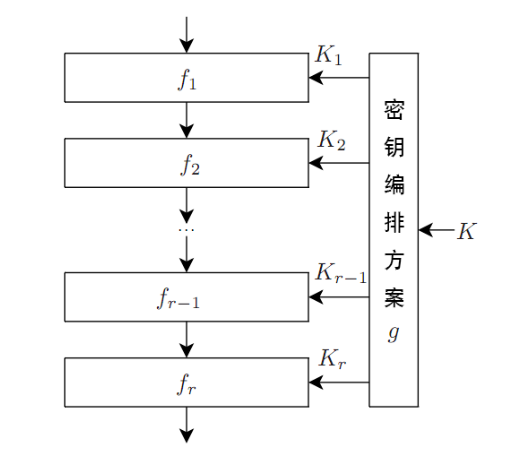
\includegraphics[width=5cm]{iterate}
    \bicaption[fig:Iterate]{迭代分组密码的一般结构}{迭代分组密码的结构}{Iterative Block Cipher}{The general structure}
\end{figure}
\begin{defn}[迭代分组密码]
    一个$r$轮的迭代分组密码$E$是一个$r$轮的带密钥置换的叠加,即:
    $$E(\cdot,k)=f_r(\cdot,k_r)\circ f_{r-1}(\cdot,k_{r-1})\circ\cdots\circ f_1(\cdot,k_1)$$
\end{defn}
其中$f_i(\cdot,k_i):\mathbb{F}^n_2\rightarrow\mathbb{F}^n_2$为第$i$轮轮函数,即依赖于轮密钥$k_i$的置换。
主密钥$K$经过密钥编排方案$g$生成$r$个轮密钥$RK_i$:
$$g:K\rightarrow(RK_1,RK_2,\dots,RK_r)$$

在一些迭代分组密码中,在第一轮轮函数开始前(或最后一轮结束后)会将明文(或密文)与一组子密钥进行异或,该组子密钥被成为白化密钥。
一般来说,为了软件和硬件上的实现效率,迭代分组密码的轮函数一般是相同的(部分密码在第一轮或最后一轮中会有些变化),因此在本文中我们会着重考虑分组密码的其中一轮的轮函数。
每一轮的轮函数一般包括三个部分:扩散层、非线性层和密钥引入层。
根据算法采用的结构不同,现有的分组密码算法结构基本可以分为三类:Feistel结构、SPN结构与Lai-Massey结构。整体结构是分组密码算法的重要特征,除了上述三种主流结构外,整体结构还包括广义(非)平衡Feistel结构、MISTY结构以及各种结构的混合使用。

\section{高级加密标准AES}
为了取代DES,Rijndael在2000年被NIST选为高级加密标准(AES),它由Daemen和Rijmen共同设计\citen{daemen2013design}。AES具有128比特的分组长度,主密钥长度支持128比特、192比特和256比特(AES-128,AES-192和AES-256),所有操作面向字节(byte-oriented)。
其中,128比特密钥版本由10轮迭代,192比特迭代12轮,256比特迭代14轮。

在AES的轮函数中,每一轮的中间状态由一个$4\times 4$的矩阵表示,该状态矩阵中每一个位置对应一个字节。$K_r$为第$r$轮的轮密钥,同样由$4\times 4$的矩阵表示。
$X^{i,j}$表示矩阵(中间状态)$X$的第$i$行第$j$列的字节。
在第一轮加密开始前,明文$P_0$和白化密钥异或;最后一轮加密中,省略列混淆操作。每一轮加密的轮函数包含以下四个步骤:
\begin{enumerate}
    \item \textbf{字节代换(SubBytes)}:并行使用16个$8\times 8$的S盒;
    \item \textbf{行移位(ShiftRows)}:状态矩阵$X$的每一行循环移位相应字节数;
    \item \textbf{列混淆(MixColumns)}:状态矩阵的每一列都和矩阵$M_{MC}$相乘(见式\ref{eq:MC});
    \item \textbf{轮密钥加(AddRoundKey)}:状态矩阵每一字节和对应轮密钥矩阵的字节进行异或。
\end{enumerate}

AES的列混淆可以矩阵$M_{MC}$表示:
\begin{equation}
    M_{MC}=\left(
    \begin{array}{cccc}
        02&03&01&01\\
        01&02&03&01\\
        01&01&02&03\\
        03&01&01&02
    \end{array}
\right)
\label{eq:MC}
\end{equation}

列混淆是一个线性变换的过程。该变换使每一个输入字节都能影响同一列的四个输出的字节,同时一个输出字节也会依赖同一行的四个输入字节。
向量和矩阵的加法和乘法均在有限域$GF(2^8)$上完成,其中$GF(2^8)$上的加法为每比特逐位异或,$GF(2^8)$的乘法为模$P(x)=x^8+x^4+x^3+x+1$的乘法。
$M_{MC}$矩阵中的元素以16进制表示一个在$GF(2)$上的多项式,如“02”表示系数为00000010的多项式。
乘以“02”即为先将$x$左移1比特,再模余式$P(x)$。 

\section{分组密码的分析方法}
对任意一个分组密码,都存在如下4种攻击方法:穷尽密钥搜索、字典攻击、查表攻击和时间-空间权衡攻击。除了这4种通用的攻击方法,在对具体的分组密码算法进行安全性分析时,往往会针对其特殊的弱点产生其他的攻击方法。
对迭代分组密码而言,密码分析者首先将寻找一个简化轮数对应算法的有效区分器,然后通过猜测区分器之外的密钥来验证区分器的正确性。
下面给出常见的几种攻击方法:
\begin{enumerate}
    \item 由Biham和Shamir在1990年针对DES算法提出的差分密码分析\cite{biham1991differential},通过观察具有特定输入差分的明文对经过加密后的密文对的差分形式来恢复密钥;
    \item 由来学家教授给出的高阶差分分析\cite{lai1994higher}是一种采用了类似高阶导数概念的差分分析法,对差分函数再求差分;
    \item Matsui提出的线性密码分析\cite{matsui1993linear},如果密码算法的输入、输出比特的某个线性组合对应一个高概率偏差的线性表达式,就可以根据这个表达式来对密码算法进行恢复密钥攻击;
    \item Diffie和Hellman提出的中间相遇攻击\cite{diffie1977special},这是一种时间-空间权衡攻击方法,是不可能差分区分器的主要寻找方法之一,本文之后会提到一个对RECTANGLE的中间相遇攻击;
    \item Knudsen基于Daemen提出的Square攻击\cite{daemen1997block}而提出的更一般形式的积分攻击\cite{knudsen2002integral};
    \item Courtoi和Pieprzyk提出的代数攻击\cite{courtois2002cryptanalysis},通过求解一个多变元的代数方程来恢复密钥;
    \item Biham和Knudsen提出的相关密钥攻击\cite{biham1994new},该密码攻击更多地考虑了密钥编排方案的性质;
    \item 由Biryukov和Wagner提出的滑动攻击\cite{biryukov1999slide},对轮函数较弱、密钥编排方案又呈周期性的迭代分组密码较为有效。
\end{enumerate}

其中中间相遇攻击、相关密钥攻击和滑动攻击可以看做是针对密钥编排方案的攻击。这些攻击无一例外利用编排方案的弱点来获得更好的攻击效果,是目前为止利用密钥编排方案弱点最有效的两种攻击手段。
